\documentclass[reportComp]{thesis}
\usepackage[cpp,pseudo]{mypackage}

\title{模式识别作业一}
\subtitle{}
\school{数据科学与计算机学院}
\author{陈鸿峥}
\classname{17大数据与人工智能}
\stunum{17341015}
\headercontext{模式识别作业}
\lstset{language=python}

\begin{document}

\maketitle

% \begin{question}[\textsection 2 Q2]
% Consider minimax criterion for the zero-one loss function, i.e., $\lambda_{11} = \lambda_{22} = 0$ and $\lambda_{12} = \lambda_{21} = 1$.
% \begin{itemize}
% 	\item [(a)] Prove that in this case the decision regions will satisfy
% \[\int_{\mathcal{R}_2}p(\vx\mid\omega_1)\diff\vx=\int_{\mathcal{R}_1}p(\vx\mid\omega_2)\diff\vx\]
% 	\item [(b)] Is this solution always unique? If not, construct a simple counterexample.
% \end{itemize}
% \end{question}
% \begin{answer}
% \end{answer}
% \begin{itemize}
% 	\item [(a)]
% 	\item [(b)]
% \end{itemize}

\begin{question}[\textsection 2 Q2]
假设两个等概率的一维密度具有如下形式:对任给$i=1,2$及$0<b_i$,$p(x\mid\omega_i)\propto\ee^{-|x-a_i|/b_i}$。
\begin{itemize}
	\item [(a)] 写出每个密度的解析表达式,即对任意的$a_i$和正的$b_i$,将每个函数归一化
	\item [(b)] 计算似然比,作为$4$个变量的函数
	\item [(c)] 绘出在$a_1=0,b_1=1,a_2=1,b_2=2$时的似然比$p(x\mid\omega_1)/p(x\mid\omega_2)$的曲线图
\end{itemize}
\end{question}
\begin{answer}
\begin{itemize}
	\item [(a)] 设比例系数为$k_i$,由概率的基本性质有
\[\begin{aligned}
\qquad&\intab{-\infty}{\infty}{k_i\ee^{\frac{-|x-a_i|}{b_i}}}\\
=&\intab{-\infty}{a_i}{k_i\ee^{\frac{x-a_i}{b_i}}}+\intab{a_i}{\infty}{k_i\ee^{-\frac{x-a_i}{b_i}}}\\
=&2k_ib_i\\\
=&1
\end{aligned}\]
进而求得$k_i=1/(2b_i)$,故解析表达式为
\[p(x\mid\omega_i)=\frac{1}{2b_i}\ee^{-|x-a_i|/b_i}\]
	\item [(b)]
\[\frac{p(x\mid\omega_1)}{p(x\mid\omega_2)}=\frac{b_2}{b_1}\ee^{-\frac{|x-a_1|}{b_1}+\frac{|x-a_2|}{b_2}}\]
	\item [(c)]
将$a_1=0,b_1=1,a_2=1,b_2=2$代入(b)求得的式子化简得
\[\frac{p(x\mid\omega_1)}{p(x\mid\omega_2)}=2\ee^{-|x|+\frac{|x-1|}{2}}\]
图像如下
\begin{figure}[H]
\centering
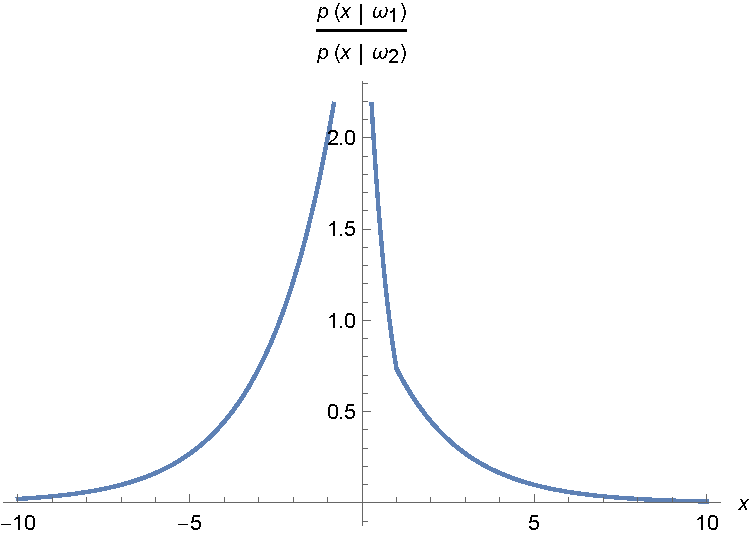
\includegraphics[width=0.5\linewidth]{likelihood.pdf}
\end{figure}
\end{itemize}
\end{answer}

\end{document}